\documentclass{mooiman_memo}
\addbibresource{./ref.bib}

\newcommand{\Dt}{\Delta t}
\renewcommand{\vec}[1]{\mbox{\boldmath $#1$} }
\newcommand{\mat}[1]{\mbox{\boldmath ${\rm #1}$} }

\begin{document}
    \memoTo{???}
    \memoConfidentialUntil{}
    \memoDate{\today~\currenttime}
    \memoVersion{001}
    \memoFrom{Jan Mooiman}
    \memoTelephone{+31\,(0)6\,4691\,4571}
    \memoEmail{jan.mooiman@outlook.com}
    \memoSubject{Two-way chemical reaction}
    \memoCopy{}

    \mooimantitle
    %------------------------------------------------------------------------------

\section{Two-way chemical reactions}
The two-way chemical reaction simulation is taken as example to see the behaviour or the fully implicit $\Delta$-formulation for reaction terms only.
This is particularly of interest for the water quality computations with lots of processes.
Example taken from \citet{HundsdorferAndVerwer2003}.

The  ODE system reads:
\begin{align}
    \pdiff{u_1}{t} & = -k_1 u_1 + k_2 u_2,
    \\
    \pdiff{u_2}{t} & = k_1 u_1 - k_2 u_2
\end{align}
with $k_1, k_2 > 0$ and initial values  $u_1(0)=0.1$ and $u_2(0) = 0.9$.
The exact solution reads:
\begin{align}
u_1(t) & =\frac{k_2}{k_1+k_2}\left( u_1(0) + u_2(0) \right)
+ \frac{\exp\left( -(k_1 + k_2)t \right)}{k_1+k_2}\left(   k_1 u_1(0) - k_2 u_2(0) \right),
\\
u_2(t) & = \frac{k_1}{k_1+k_2}\left( u_1(0) + u_2(0) \right)
- \frac{\exp\left( -(k_1 + k_2)t \right)}{k_1+k_2}\left(   k_1 u_1(0) - k_2 u_2(0) \right).
\end{align}
after a short time the term $\exp\left( -(k_1 + k_2)t \right)$ is negligible.

%
%
Some results are:
\begin{figure}[H]
    \begin{subfigure}{0.49\textwidth}
        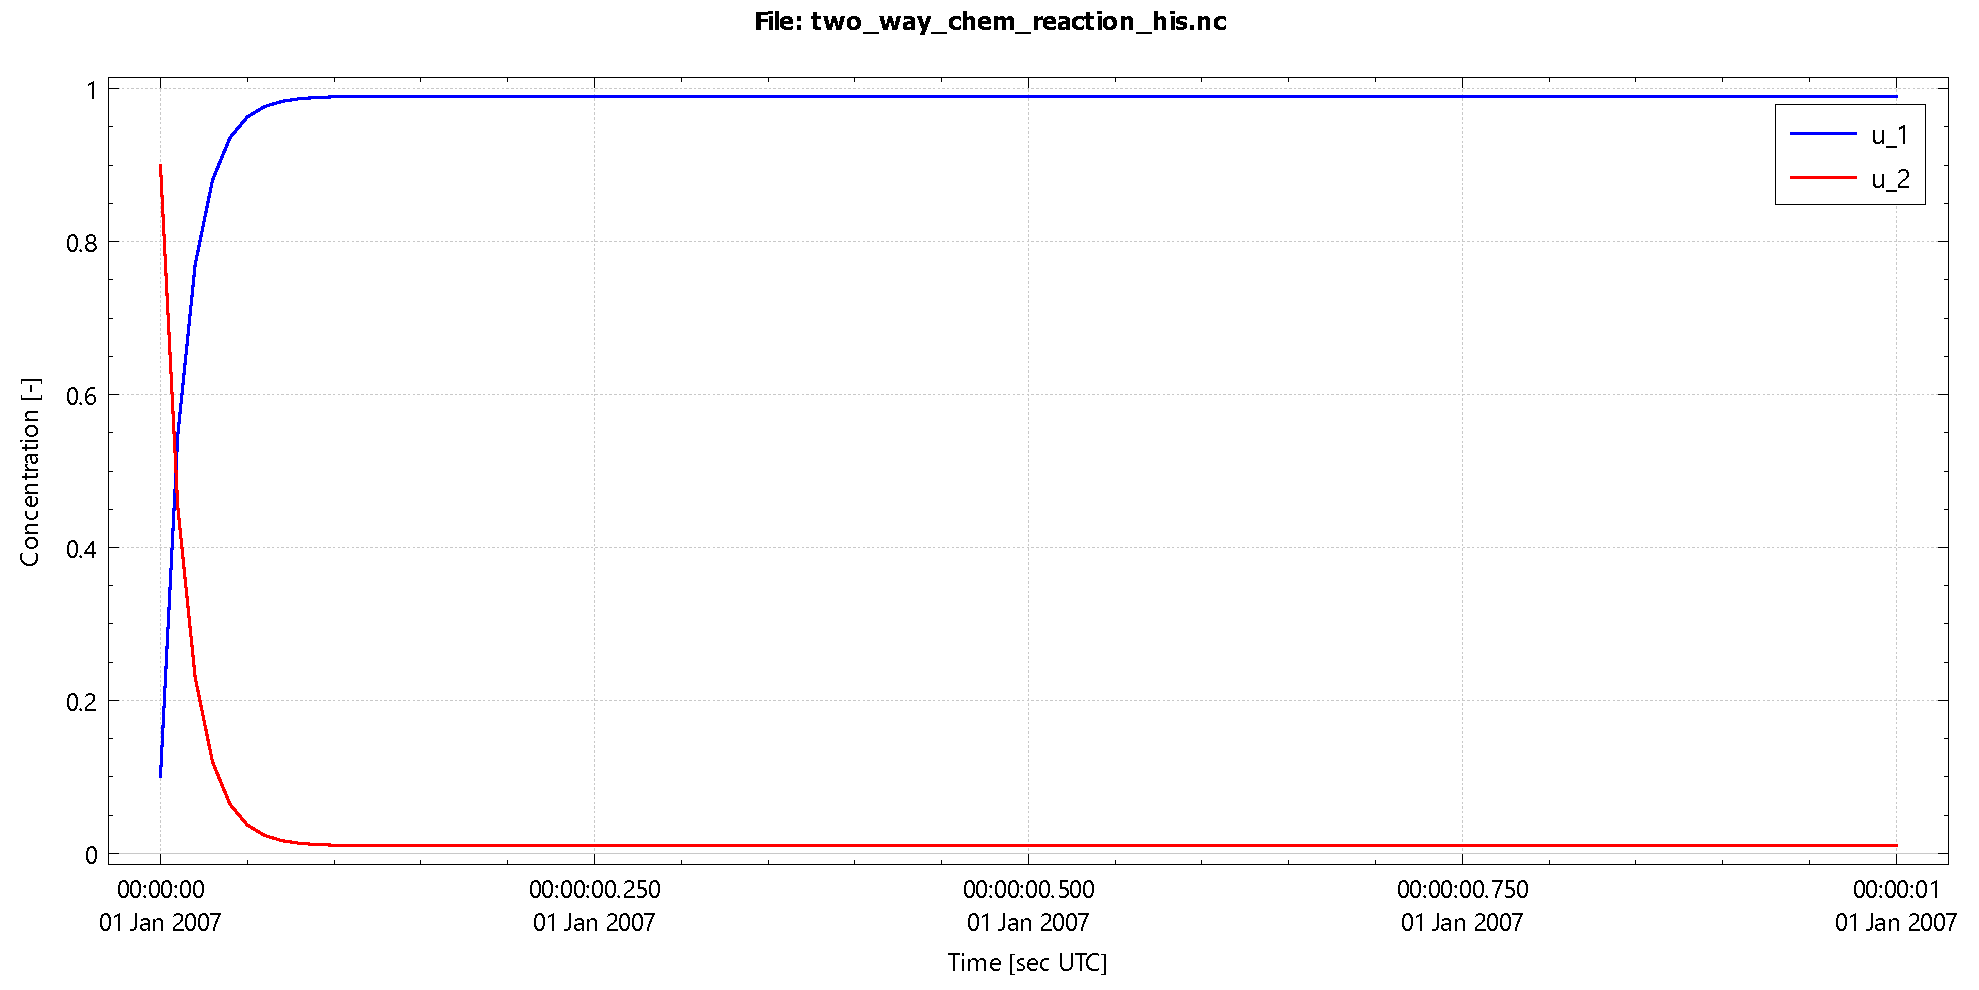
\includegraphics[width=\textwidth]{figures/two_way_chem_reaction_imp_dt=0d01.pdf}
        \caption{Fully Implicit: $\Dt=0.01$, $k_1=1$, $k_2=100$}\label{fig:imp_dt=1d00}
    \end{subfigure}
    \hfill
    \begin{subfigure}{0.49\textwidth}
        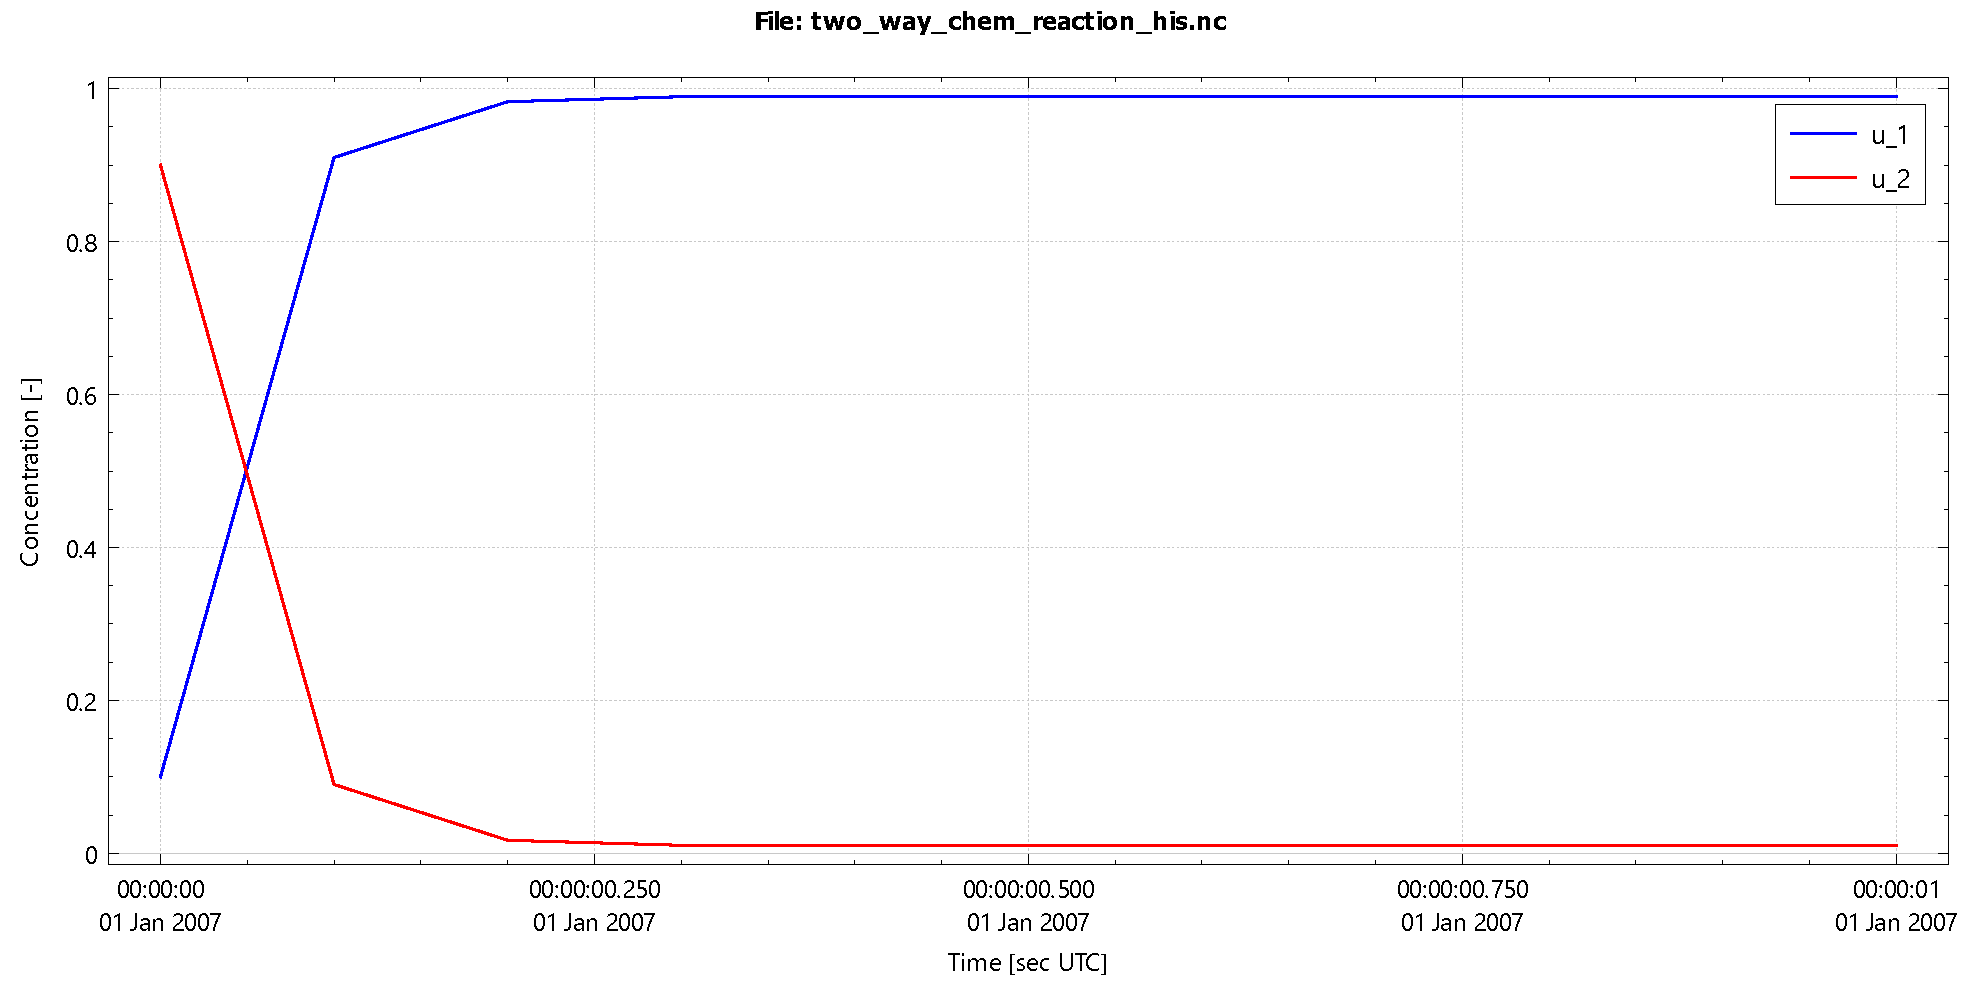
\includegraphics[width=\textwidth]{figures/two_way_chem_reaction_imp_dt=0d10.pdf}
        \caption{Fully Implicit: $\Dt=0.1$, $k_1=1$, $k_2=100$}\label{fig:imp_dt=5d00}
    \end{subfigure}
    \caption{Result plots for constant value of $k_1 = 1$ and $k_2 =100$, computed with a fully implicit ($\Delta$-formulation) time integration method for different time steps $\Dt = 0.01, 0.1 [s]$.
    }
\end{figure}
%
%%-------------------------------------------------------------------------------
\section{Numerics}
Discretized
\begin{align}
    \frac{1}{\Dt}\Delta u_1^{n+1, p+1} & = - \frac{1}{\Dt}(u_1^{n+1,p} - u_1^n) - k_1 (u_1^{n+\theta,p+1}) + k_2 (u_2^{n+\theta,p+1})
    \\
    \frac{1}{\Dt}\Delta u_2^{n+1, p+1} & = - \frac{1}{\Dt}(u_2^{n+1,p} - u_2^n) + k_1(u_1^{n+\theta,p+1}) - k_2 (u_2^{n+\theta,p+1})
\end{align}
Linearization of $\vec{u}^{n+\theta,p+1}$:
\begin{align}
    \frac{1}{\Dt}\Delta u_1^{n+1, p+1} & =
    - \frac{1}{\Dt}(u_1^{n+1,p} - u_1^n) + \\
    & - k_1 (u_1^{n+\theta,p} + \theta \Delta u_1^{n+1, p+1})
      + k_2 (u_2^{n+\theta,p} + \theta \Delta u_2^{n+1, p+1})
    \\
    \frac{1}{\Dt}\Delta u_2^{n+1, p+1} & = - \frac{1}{\Dt}(u_2^{n+1,p} - u_2^n) +
    \\
    & + k_1 (u_1^{n+\theta,p} + \theta \Delta u_1^{n+1, p+1})
      - k_2 (u_2^{n+\theta,p} + \theta \Delta u_2^{n+1, p+1})
\end{align}
Rearrange to $\mat{A}\vec{x}=\vec{b}$
\begin{align}
    \frac{1}{\Dt}\Delta u_1^{n+1, p+1} & + k_1 \theta \Delta u_1^{n+1, p+1} - k_2 \theta \Delta u_2^{n+1, p+1} =
    \\
& = - \frac{1}{\Dt}(u_1^{n+1,p} - u_1^n) - k_1 u_1^{n+\theta,p} + k_2 u_2^{n+\theta,p}
\\
\frac{1}{\Dt}\Delta u_2^{n+1, p+1} & - k_1 \theta \Delta u_1^{n+1, p+1} + k_2 \theta \Delta u_2^{n+1, p+1} = \\
& =- \frac{1}{\Dt}(u_2^{n+1,p} - u_2^n) + k_1 u_1^{n+\theta,p}
- k_2 u_2^{n+\theta,p}
\end{align}
%
%
%------------------------------------------------------------------------------
\section{Numerical experiment}
Data used from the values mentioned in the previous sections.
%
\begin{longtable}{>{\bfseries}p{6mm-12pt}|p{\textwidth/3-2mm-12pt}|p{\textwidth/3-2mm-12pt}|p{\textwidth/3-2mm-12pt}}
\caption{Stability of different time integrators for the Two-way chemical reaction.}\\%
\rowcolor{kobaltblue}
& {\textcolor{white}{\textbf{Time step\newline [s]}}}
& {\textcolor{white}{\textbf{Runge-Kutta 4}}}
& {\textcolor{white}{\textbf{Fully Implicit\newline $\Delta$-formulation}}}
\\
\topline
\endfirsthead
\rowcolor{kobaltblue}
& {\textcolor{white}{\textbf{Time step\newline [s]}}}
& {\textcolor{white}{\textbf{Runge-Kutta 4}}}
& {\textcolor{white}{\textbf{Fully Implicit\newline $\Delta$-formulation}}}
\\
\midline
\endhead
\endfoot
\endlastfoot
1 & 0.01 & \checkmark & \checkmark  \\
\midline
2 & 0.1  & unstable &  \checkmark   \\
\bottomline
\end{longtable}
%

%------------------------------------------------------------------------------
\printallbibliography
\end{document}
